\documentclass[svgnames,final]{beamer}
\usepackage{etex}
\mode<presentation> {
  \usetheme{I6dv}
}
\usepackage[utf8]{inputenc}
%\usepackage[T1]{fontenc}
\usepackage[english]{babel}
\usepackage{amsmath,amsfonts,amsthm}
\usepackage{mathtools}
\usepackage{booktabs}
\usepackage[orientation=landscape,size=a0,scale=1.4]{beamerposter}
\usepackage{pgfplots}
\usepackage{comment}
% \usepackage{algorithm}
\usepackage[noend]{algpseudocode}
\usepackage{etoolbox}
\pgfplotsset{compat=1.12}
\usepackage{tikz}
\usetikzlibrary{positioning,plotmarks,calc,arrows,decorations.markings,intersections,backgrounds}
\usepackage{subcaption}
\usepackage{amsmath,amsfonts,amsthm,bm} % Math packages


\newcommand{\thetatilde}{\ensuremath{\tilde{\theta}}}
%\tikzexternalize[prefix=tikz_output/]

\usepackage [english]{babel}
\usepackage [autostyle, english = american]{csquotes}
\MakeOuterQuote{"}

\newtoggle{plotexperiments}
\toggletrue{plotexperiments}
%\togglefalse{plotexperiments}

\newcommand{\numplotsamples}{200}

\newcommand{\red}[1]{\textcolor{red}{#1}}
\newcommand{\green}[1]{\textcolor{Green}{#1}}
\newcommand{\blue}[1]{\textcolor{blue}{#1}}
\newcommand{\eps}{\ensuremath{\epsilon}}
\newcommand{\R}{\ensuremath{\mathbb{R}}}
\newcommand{\setC}{\ensuremath{\mathcal{C}}}
\newcommand{\thetahat}{\ensuremath{\hat{\theta}}}
\newcommand{\thetastar}{\ensuremath{\theta^*}}
\newcommand{\Otilde}{\ensuremath{\widetilde{O}}}
\newcommand{\OPT}{\ensuremath{\textnormal{OPT}}}
\newcommand{\projH}{\ensuremath{\mathcal{H}}}
\newcommand{\projT}{\ensuremath{\mathcal{T}}}
\newcommand{\Usubspaces}{\ensuremath{\mathbb{U}}}
\DeclarePairedDelimiter{\abs}{\lvert}{\rvert}
\DeclareMathOperator*{\argmin}{arg\,min}
\DeclarePairedDelimiter{\norm}{\lVert}{\rVert}
\newcommand{\specialcell}[2][c]{%
  \begin{tabular}[#1]{@{}c@{}}#2\end{tabular}}

\newcommand{\prospoint}[1]{\textcolor{Green}{Pros: #1}}
\newcommand{\conspoint}[1]{\textcolor{red}{Cons: #1}}

\newcommand{\greencell}[1]{\green{#1}}
\newcommand{\redcell}[1]{\red{#1}}
\newcommand{\yellowcell}[1]{\textcolor{orange!40!yellow}{#1}}

\title{Graph-Sparse Logistic Regression}
\author{Alexander LeNail$^1$, Ludwig Schmidt$^2$, Jonathan Li$^1$, Tobias Ehrenberger$^1$, Karen Sachs$^1$, Stefanie Jegelka$^2$, Ernest Fraenkel$^1$}
\institute{$^1$MIT BE, $^2$MIT CSAIL}

\begin{document}

\begin{frame}
\vspace{-.5cm}
\begin{columns}[T]

\begin{column}{.3\linewidth}

	%%%%%%%%%%%%%%%%%%%%%%%%%%%%%%%%%%%%%%%%%%%%%%%%%%%%%%%%%%%%%%%%%%%%%%%%%%%
	\begin{block}{Problem setup}
    \textbf{Variable selection} in a linear model:
    {\Large
    \[
      y \; = \; \sigma(X \,  \thetastar + e)
    \]
    }

		\textbf{Scientists} often use machine learning to \textbf{learn more about their data},
		not to predict it. They want to \textbf{interpret} their models. \\

		The simplest way to build an interpretable model is to keep it \textbf{small}.
		The classic way to accomplish this is with \textbf{LASSO} (L1-regularization).

	\end{block}

	\vspace{2cm}

	%%%%%%%%%%%%%%%%%%%%%%%%%%%%%%%%%%%%%%%%%%%%%%%%%%%%%%%%%%%%%%%%%%%%%%%%%%%
	\begin{block}{Problem setup}

		The LASSO does not always find the "right" model. In some cases,
		we can leverage side-information to help find the right model.

		\vspace{.5cm}

		In our case, side-information is graphical structure among the features.

		\begin{figure}[h]
		\centering
		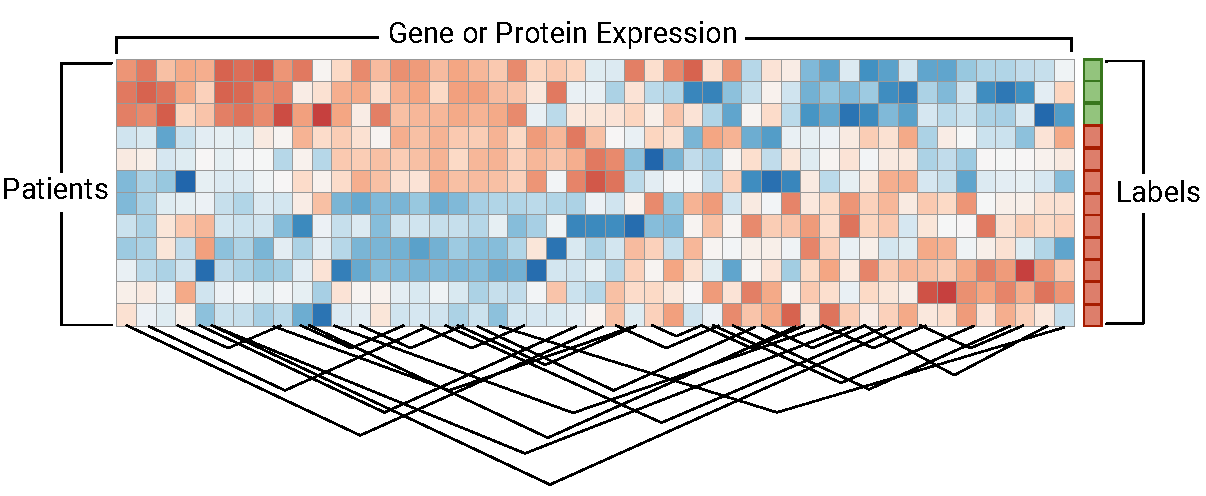
\includegraphics[width=\linewidth]{images/matrix.pdf}
		\end{figure}

		We can re-draw each instance as a labeling of the graph's nodes:

		\begin{figure}[h]
		\centering
		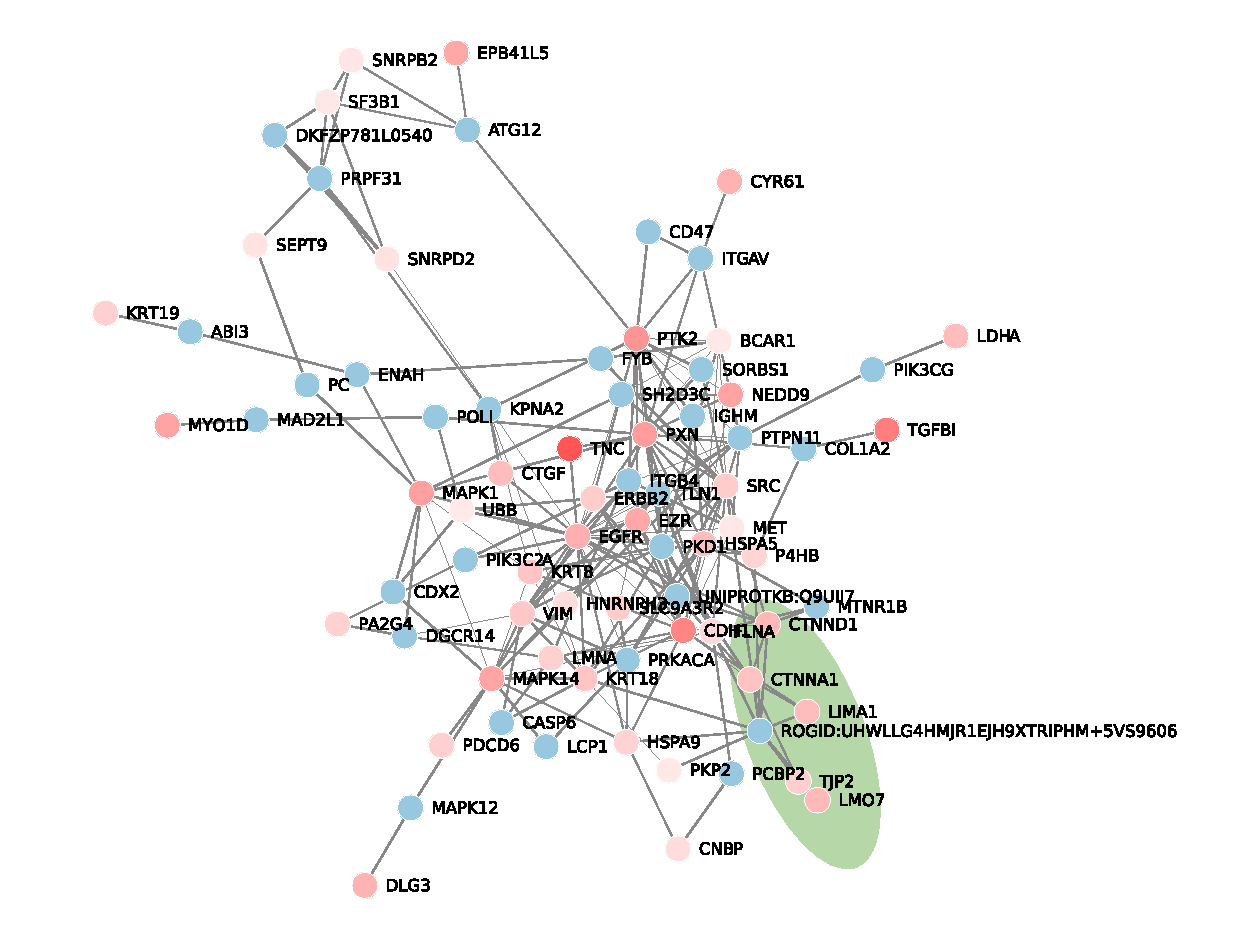
\includegraphics[width=0.8\linewidth]{images/graph.pdf}
		\end{figure}

		The "right" model is a "graph-sparse" model, i.e. a model with a sparse support which is connected on a graph.
		The goal is therefore to find the \textbf{most predictive connected subgraph}.

		(possibly add the logistic loss function here?)

	\end{block}

	\vspace{2cm}

\end{column}

\begin{column}{.3\linewidth}

	%%%%%%%%%%%%%%%%%%%%%%%%%%%%%%%%%%%%%%%%%%%%%%%%%%%%%%%%%%%%%%%%%%%%%%%%%%%
	\begin{block}{Our approach}

		% \begin{algorithm}
		% \caption{Graph-Sparse Logistic Regression}
		% \label{alg:gslr}
		\begin{algorithmic}%[1]
		\Function{GSLR}{$X$, $y$, $G$, $s$, $\eta$, $k$}
		\State Let $f(X, y, \theta)$ be the logistic loss.
		\State $\thetahat^0 \gets 0$
		\For{$i \gets 0, \ldots, k-1$}
		\State $\thetatilde^{i+1} \gets \thetahat^i - \eta \cdot \nabla f(X, y, \thetahat^i)$
		\State $\thetahat^{i+1} \gets P_{G,s}(\thetatilde^{i+1})$ \Comment{Graph-sparse projection}
		\EndFor
		\State \textbf{return} $\thetahat^k$
		\EndFunction
		\end{algorithmic}
		% \end{algorithm}


		\vspace{2cm}

		\textbf{Main idea:}

		\begin{figure}[h]
		\centering
		
\includegraphics[width=\linewidth]{images/algo.pdf}
		\label{fig:test}
		\end{figure}


		\vspace{2cm}

		\textbf{Sparse Projection Operator:}

		Given an arbitrary vector $p \in \R^d$, the projection operator $P_{G,s}$
		returns a vector $q \in \R^d$ satisfying the following two properties:
		\begin{itemize}
		\item \textbf{Approximate projection:} The vector $q$ is an approximate projection,
					i.e., instead of achieving the smallest distance to the input point $p$ among points in the constraint set,
					the distance achieved by $q$ is within a small constant factor:
		\begin{equation}
		\label{eq:approxproj}
		  \|p - q \|_2^2  \; \leq \; 2 \cdot \min_{q' \textnormal{ is } (G,s)\textnormal{-sparse}} \| p - q'\|_2^2 \; .
		\end{equation}
		\item \textbf{Approximate graph sparsity:} The support of the vector $q$ forms
					a connected component of size at most $6s + 1$ in the graph $G$.
		\end{itemize}


		\vspace{2cm}

		\textbf{Graph-Sparse Projection through PCSF:}

		The Graph-Sparse projection operator $P_{G,s}$ is a carefully-tuned set of Prize-Collecting Steiner Forest instances.

		The PCSF objective is to minimize:

		\begin{equation}
			f(F) = \beta \sum_{v\notin V_F} p(v) + \sum_{e\in E_F} c(e) + \omega \cdot \kappa,
		\end{equation}

		Intuitively, the goal is to pay as little edge cost to connect the highest prize nodes.

		We project the parameter vector $theta$ onto the graph by setting it as the prize for PCSF.



	\end{block}
\end{column}

\begin{column}{.3\linewidth}

	%%%%%%%%%%%%%%%%%%%%%%%%%%%%%%%%%%%%%%%%%%%%%%%%%%%%%%%%%%%%%%%%%%%%%%%%%%%
	\begin{block}{Experimental Setup}

		Since we don't have the ground truth subgraphs for the real data, \\
		we generate synthetic data by this procedure:

		1. Determine $\mu$ and $\bm{\Sigma}$ from real data.

		2. Sample from multivariate $\mathcal{N} (\vec{\mu}, \bm{\Sigma} )$

		3. Sample perturbation vector $\vec{x}$:

			\setlength\parindent{96pt}

			scheme 1: $\vec{x_p} = \mathcal{N} (0, \sigma_p^2 )$ if $p \in$ KEGG, 0 otherwise

			scheme 2: $\vec{x_p} = \mathcal{N} (\pm\sigma_p, \sigma_p^2 )$ if $p \in$ KEGG, 0 otherwise

			\setlength\parindent{0pt}

		4. Translate "positive" samples by perturbation vector


		\begin{figure}[h]
		  \centering
		\begin{tikzpicture}[
		declare function={mu1=1;},
		declare function={mu2=2;},
		declare function={mu3=2;},
		declare function={sigma1=0.5;},
		declare function={sigma2=1;},
		declare function={normal(\m,\s)=1/(2*\s*sqrt(pi))*exp(-(x-\m)^2/(2*\s^2));},
		declare function={bivar(\ma,\sa,\mb,\sb)=3.3/(2*pi*\sa*\sb) * exp(-((x-\ma)^2/\sa^2 + (y-\mb)^2/\sb^2))/2;}]
		\begin{axis}[
		ticks=none,
		colormap name=whitered,
		width=18cm,
		view={35}{65},
		enlargelimits=false,
		grid=major,
		domain=-1:4,
		y domain=-1:4,
		samples=26,
		xlabel=$x_1$,
		ylabel=$x_2$,
		zlabel={$P$},
		]

		\addplot3 [opacity=1,surf,colormap={whitered}{color(0cm)=(white); color(1cm)=(orange!75!red)}] {bivar(mu1,sigma1,mu2,sigma2)};
		\addplot3 [opacity=0.5,surf,colormap={whiteyellow}{color(0cm)=(white); color(1cm)=(orange!75!yellow)}] {bivar(mu3,sigma1,mu2,sigma2)};

		\addplot3 [domain=-1:4,samples=31, samples y=0, thin, smooth] (x,4,{normal(mu1,sigma1)});
		\addplot3 [domain=-1:4,samples=31, samples y=0, thin, smooth] (-1,x,{normal(mu2,sigma2)});
		\addplot3 [domain=-1:4,samples=31, samples y=0, thin, smooth] (x,4,{normal(mu3,sigma1)});

		\draw [black!50] (axis cs:-1,0,0) -- (axis cs:4,0,0);
		\draw [black!50] (axis cs:0,-1,0) -- (axis cs:0,4,0);

		\end{axis}
		\end{tikzpicture}
		\end{figure}


		Since we know the perturbation vector, we know the ground truth!

		We can then evaluate algorithms on the feature selection task.

	\end{block}


	%%%%%%%%%%%%%%%%%%%%%%%%%%%%%%%%%%%%%%%%%%%%%%%%%%%%%%%%%%%%%%%%%%%%%%%%%%%
	\begin{block}{Experimental Results}

		We benchmark our technique against the LASSO by how many of the truly "perturbed" features each uses in its support.

		\begin{figure}[h]
		\centering
		\begin{subfigure}{.5\textwidth}
		  \centering
		  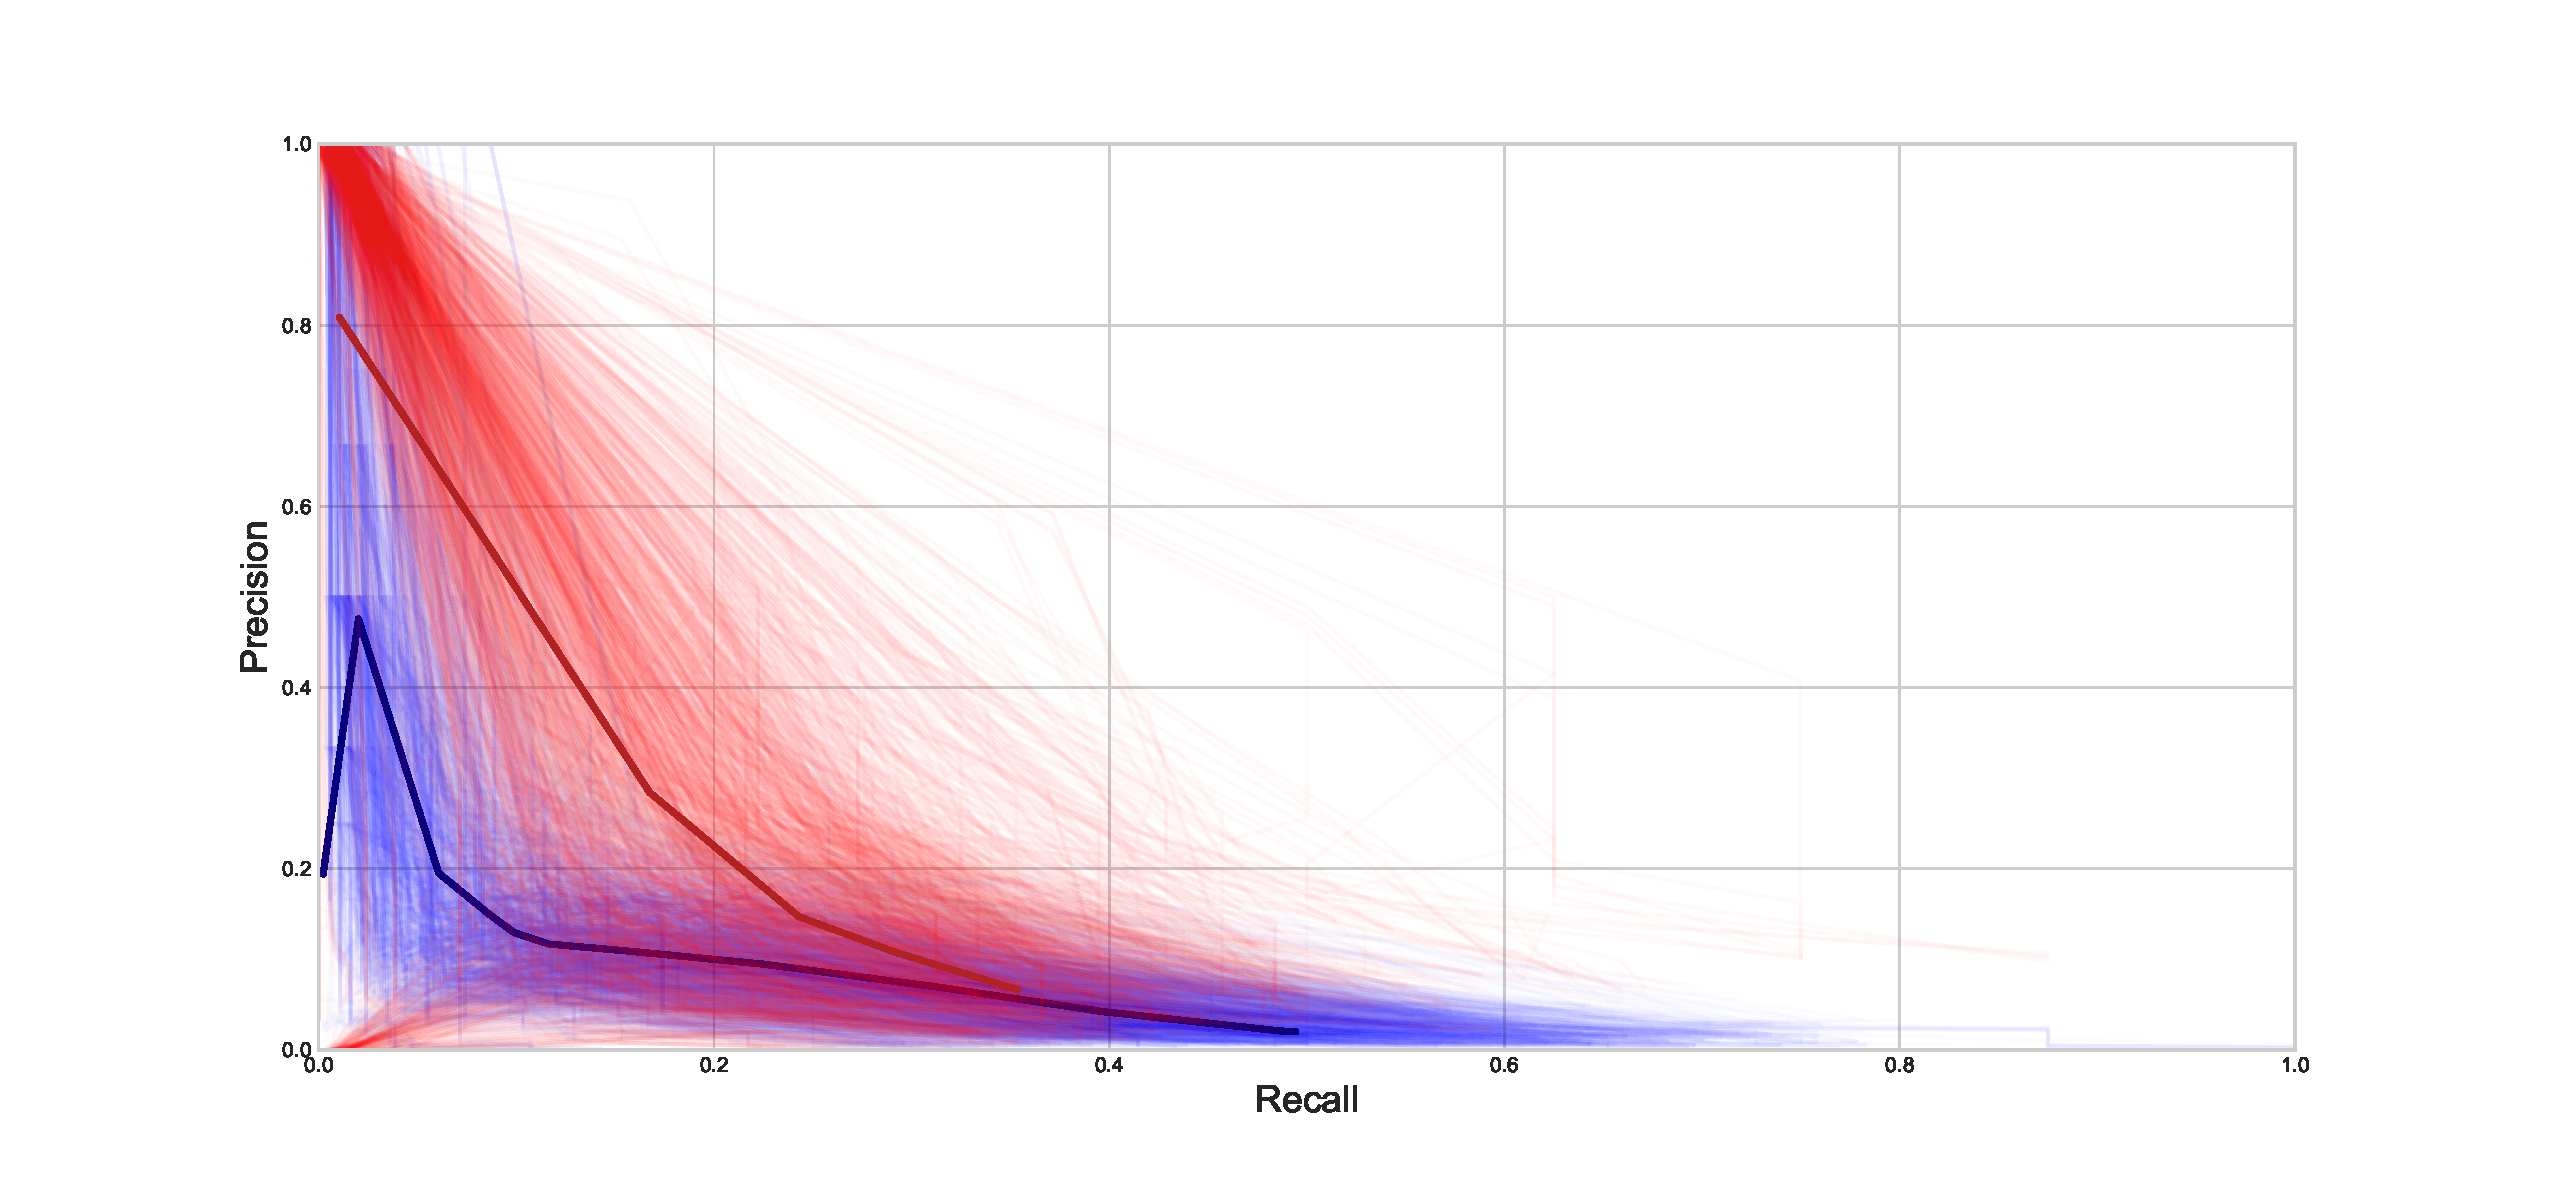
\includegraphics[width=\linewidth]{images/2.pdf}
		  \label{fig:sub1}
		\end{subfigure}%
		\begin{subfigure}{.5\textwidth}
		  \centering
		  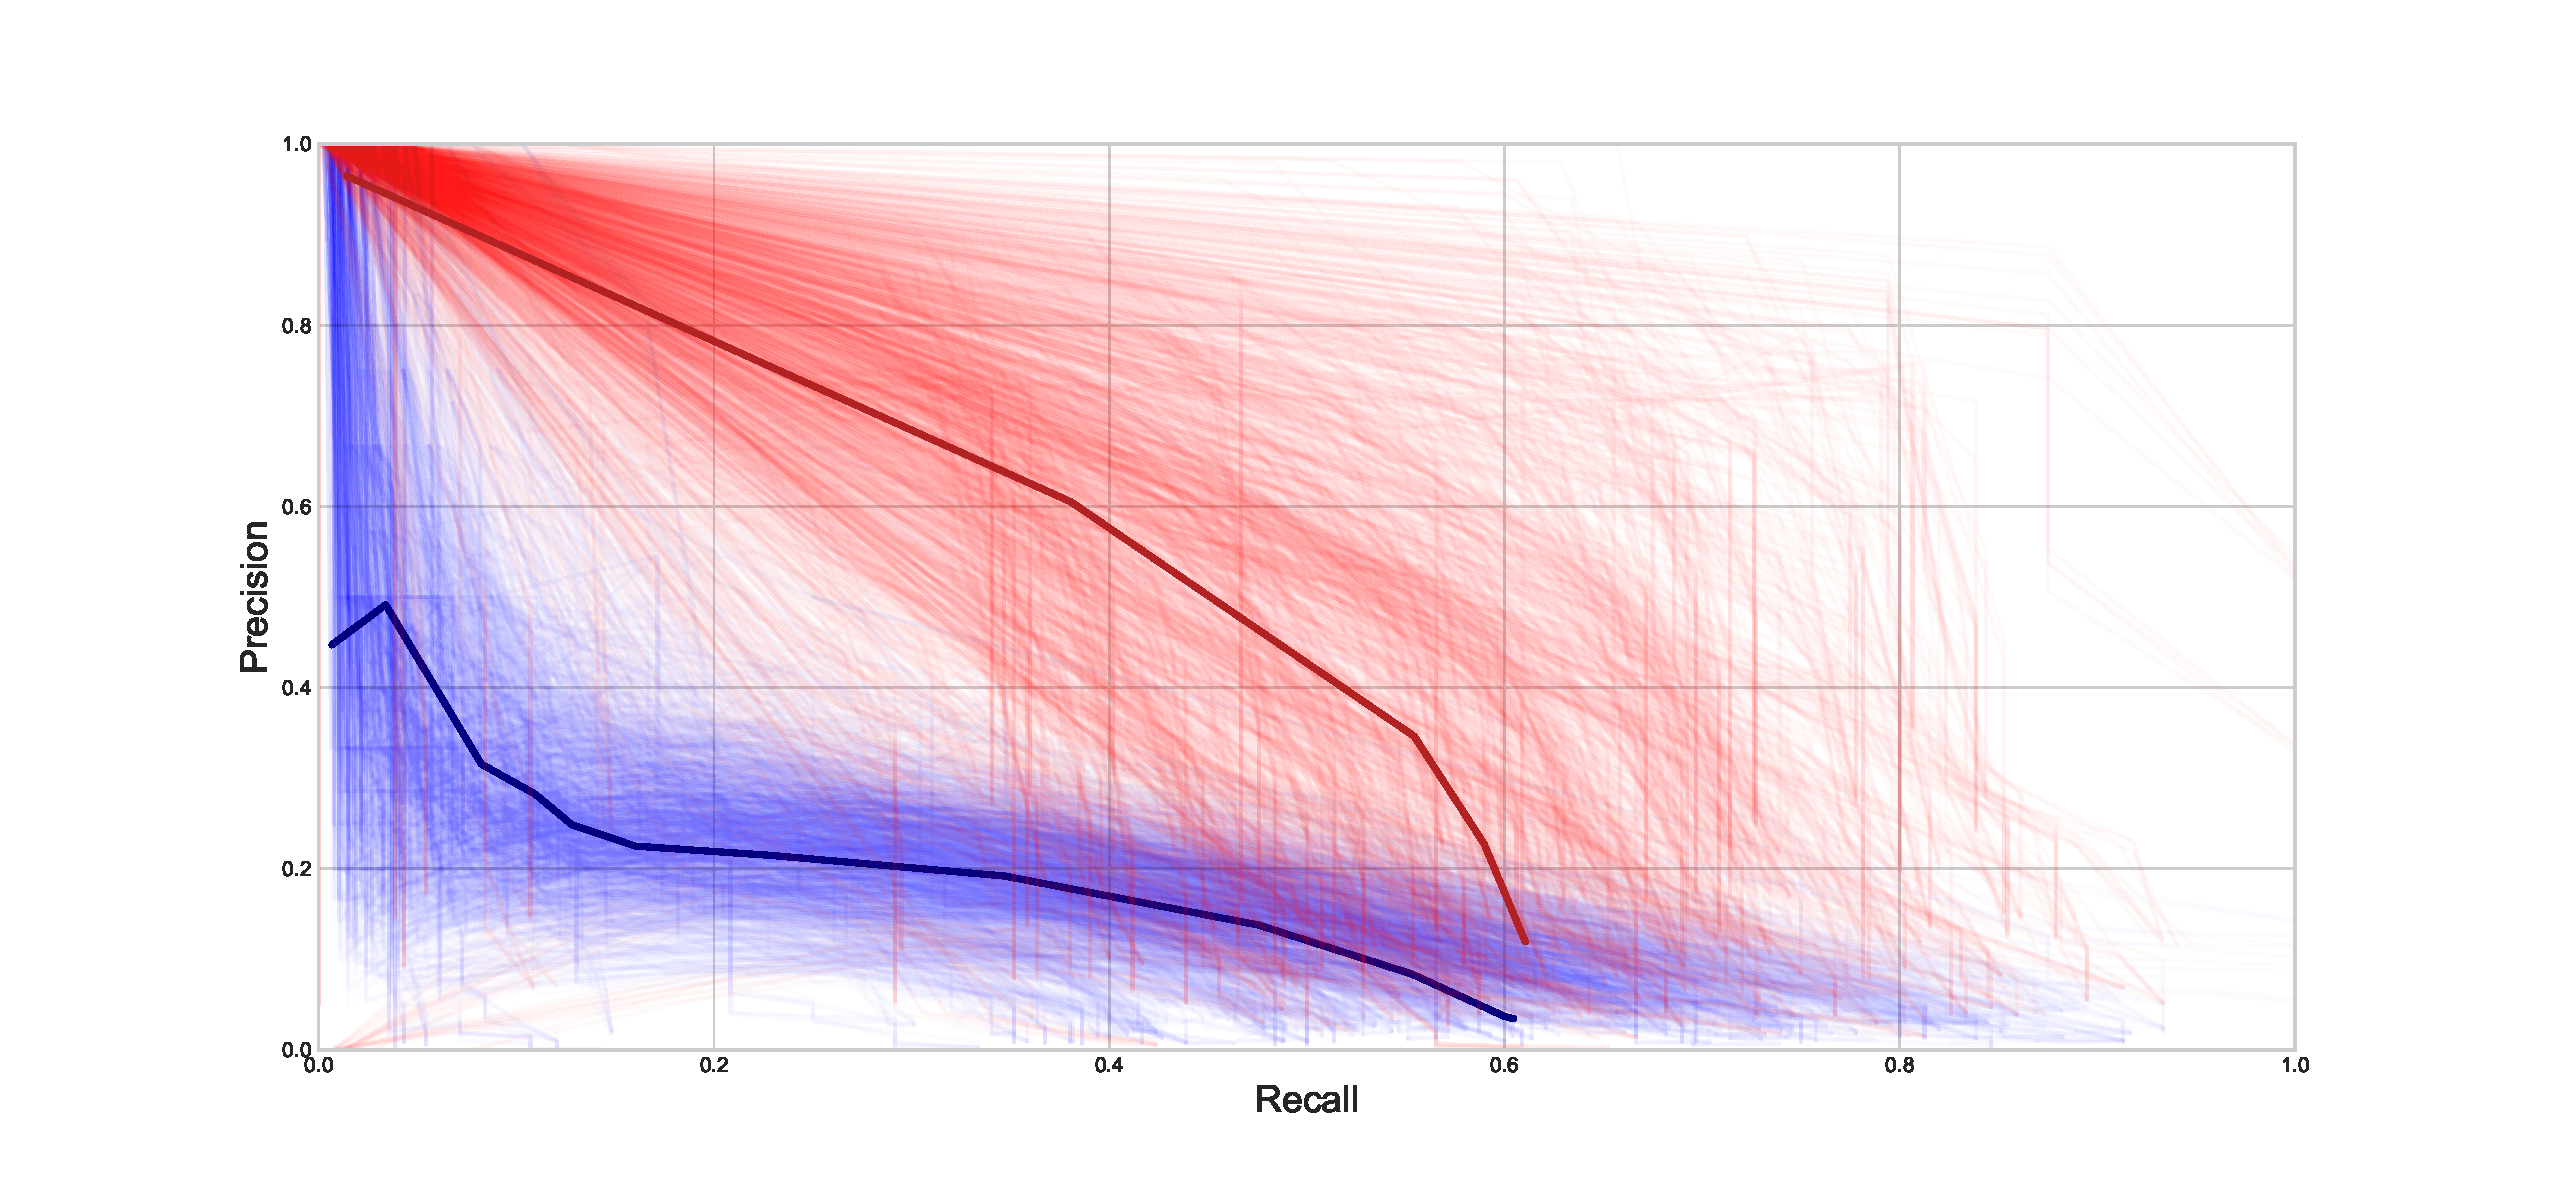
\includegraphics[width=\linewidth]{images/1.pdf}
		  \label{fig:sub2}
		\end{subfigure}
		\begin{subfigure}{.5\textwidth}
		  \centering
		  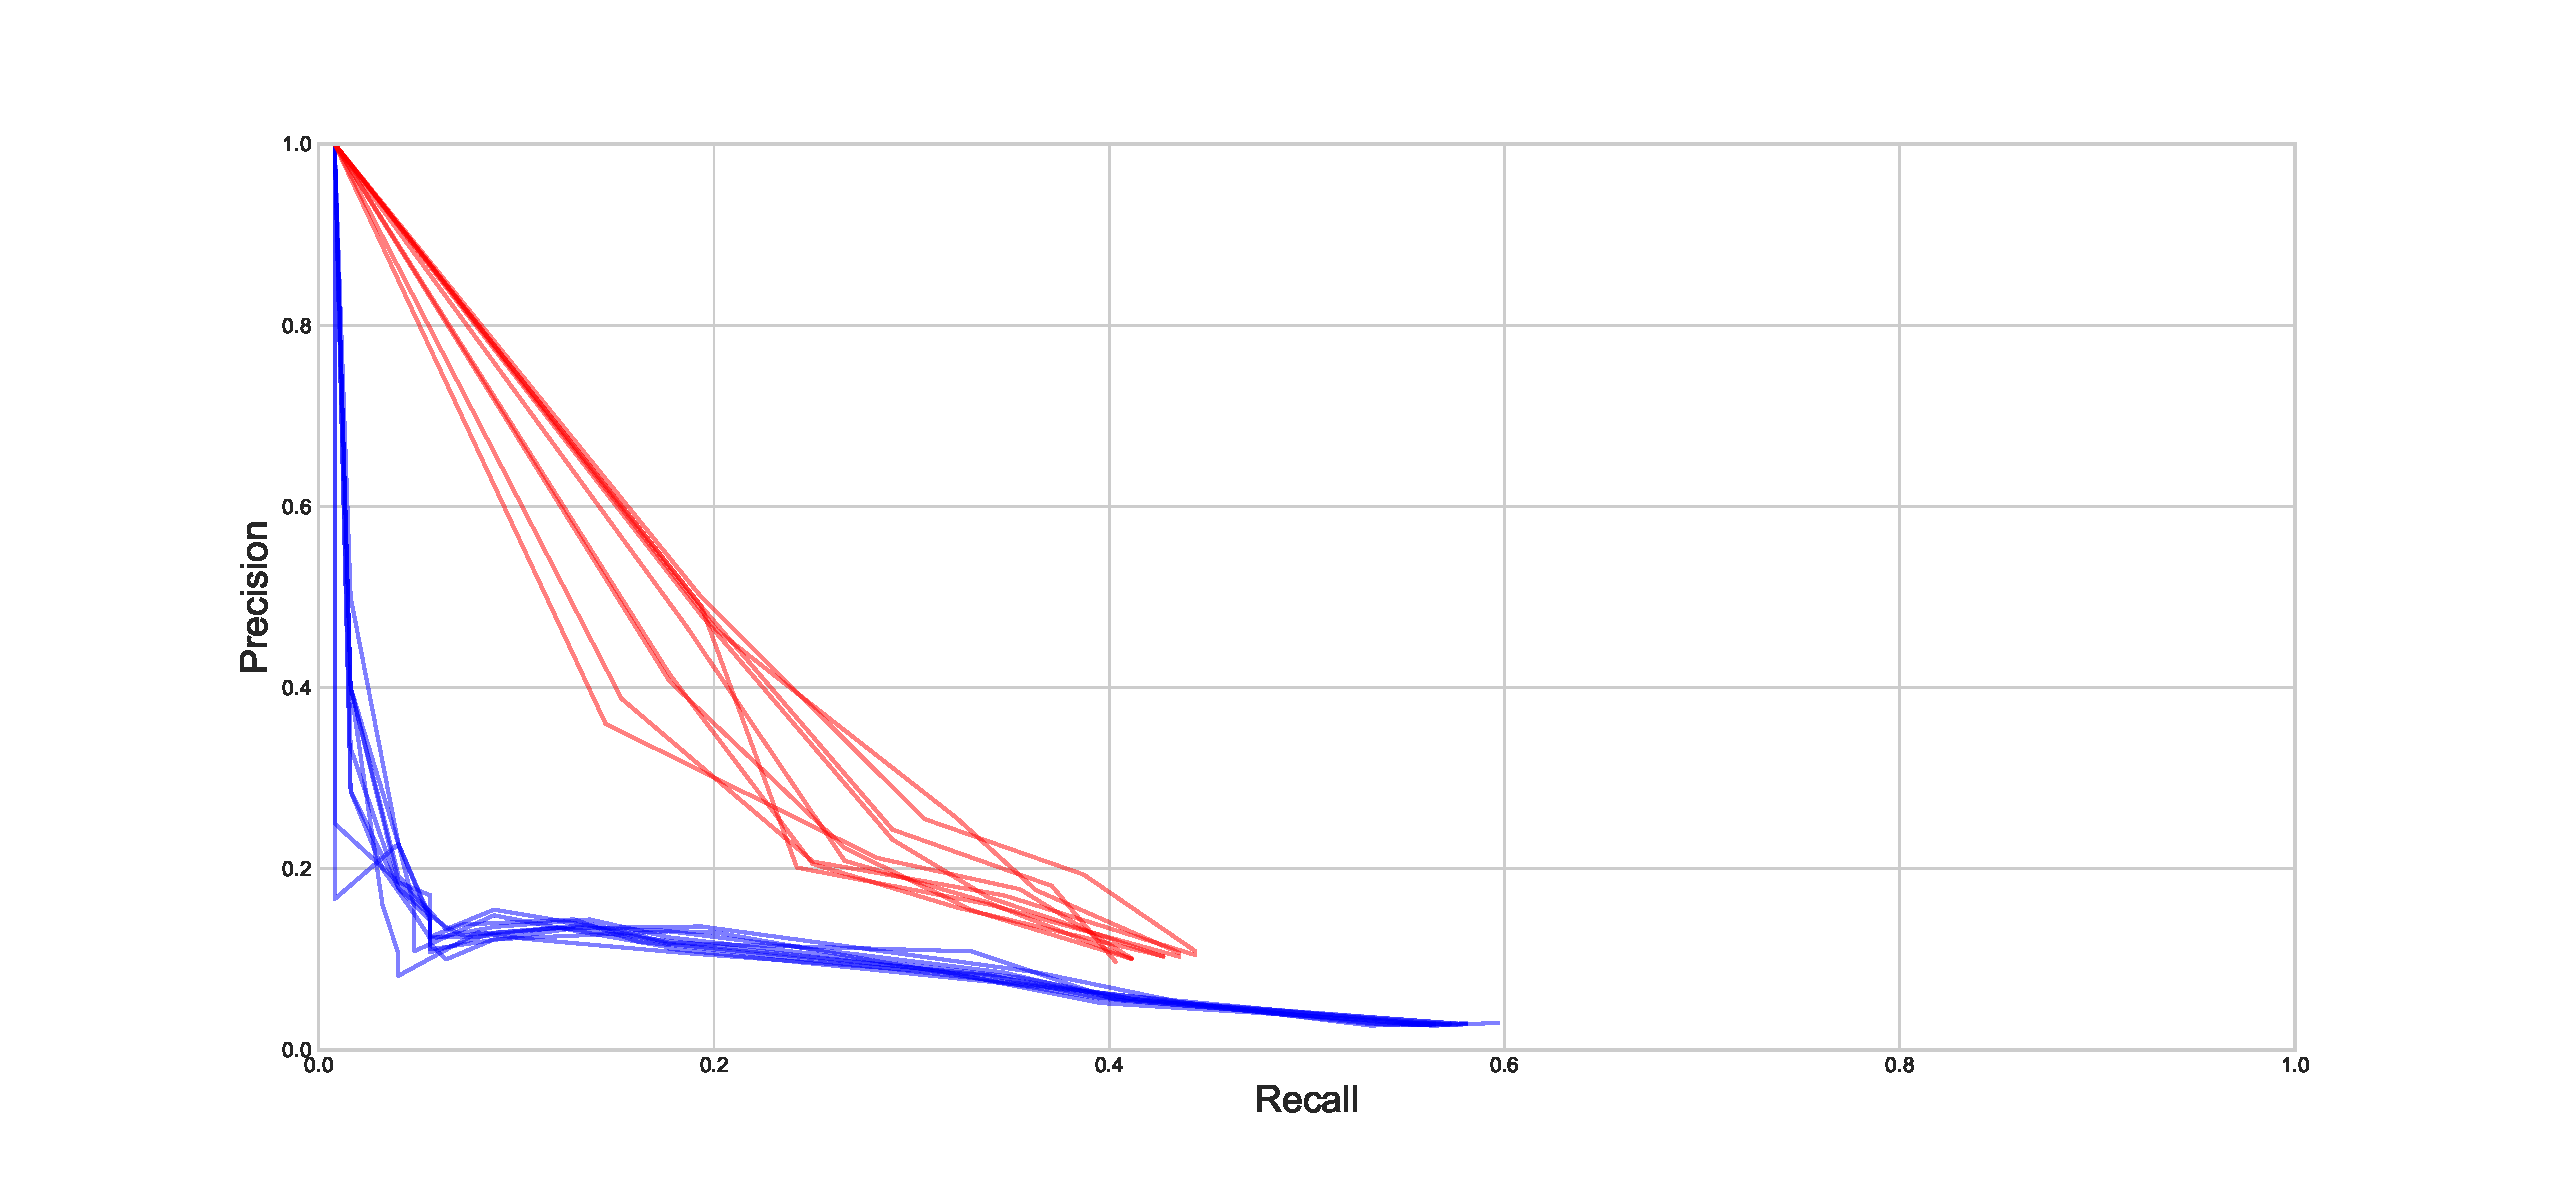
\includegraphics[width=\linewidth]{images/4.pdf}
		  \label{fig:sub3}
		\end{subfigure}%
		\begin{subfigure}{.5\textwidth}
		  \centering
		  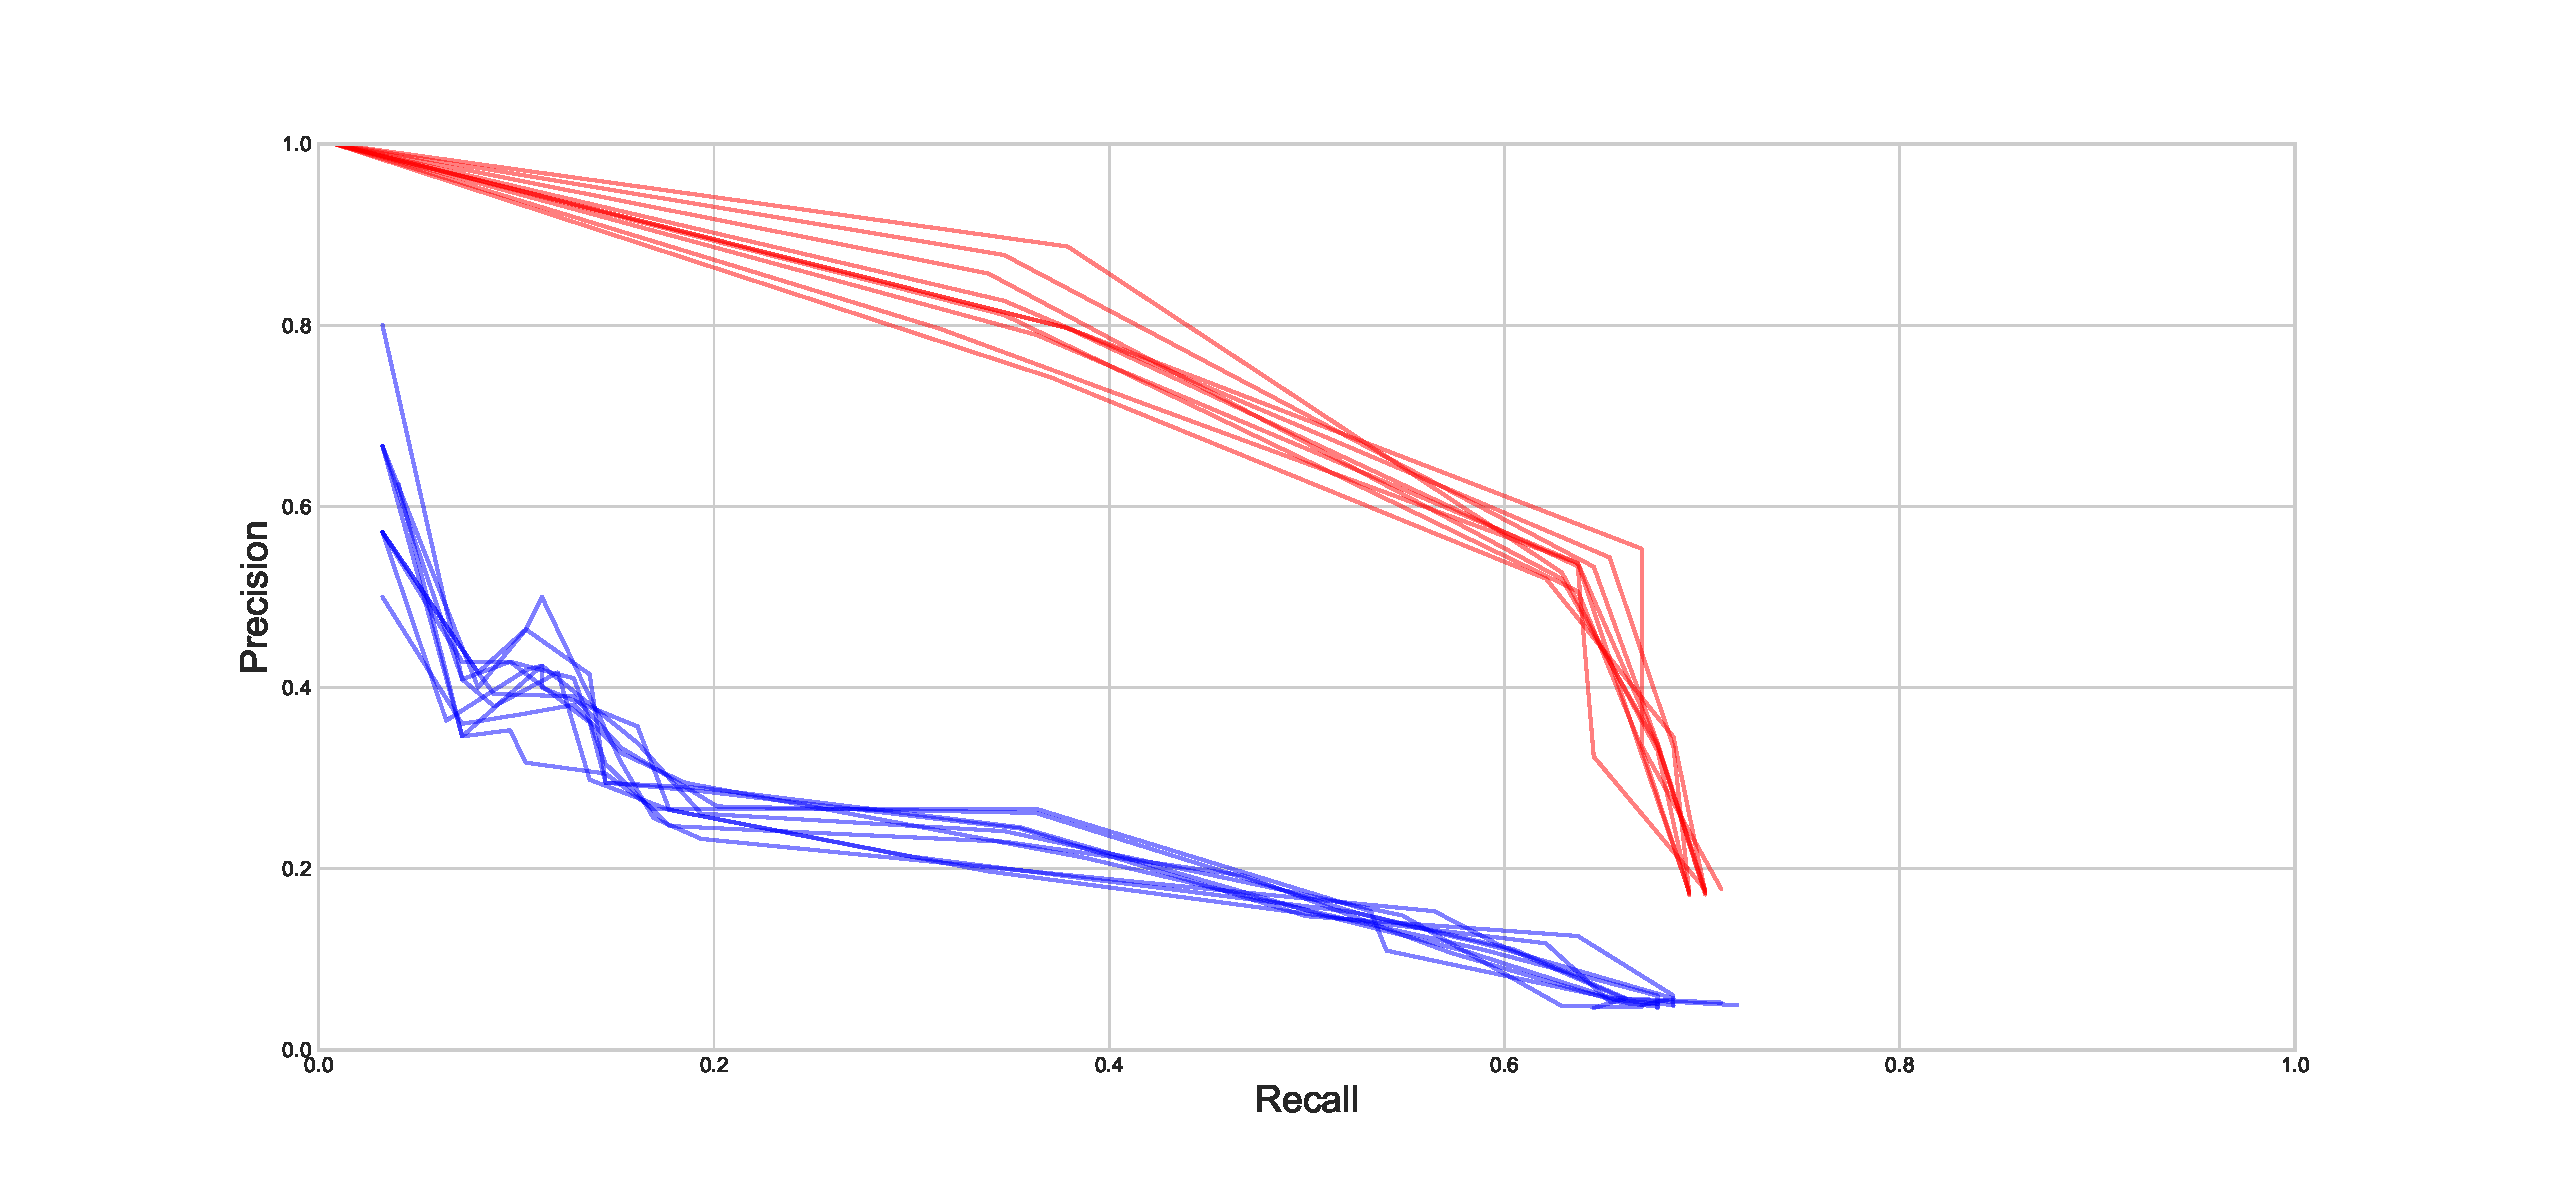
\includegraphics[width=\linewidth]{images/3.pdf}
		  \label{fig:sub4}
		\end{subfigure}
		\label{fig:perf}
		\end{figure}

		We then use our technique on real Ovarian Cancer data,
		and find that the support chosen by GSLR is qualitatively superior.

	\end{block}

	\vspace{2cm}

	% %%%%%%%%%%%%%%%%%%%%%%%%%%%%%%%%%%%%%%%%%%%%%%%%%%%%%%%%%%%%%%%%%%%%%%%%%%%
	% \begin{block}{Conclusion}



	% \end{block}

\end{column}
\end{columns}
\end{frame}
\end{document}
